\section{Resultate}
\subsection{DSL}
\begin{code}
	\caption{ProjectGeneratorQuickfixProvider.xtend}
	\javaSourceFile{\imageDir/evaluation.moduledsl}
	\label{src:module-dsl}
\end{code}

\subsection{Validierung und Quickfix}
\begin{figure}[h]
	\centering
	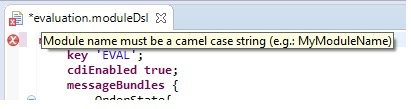
\includegraphics[scale=0.9]{\imageDir/validation-module-name-camel.jpg}
	\caption{Modulname muss \emph{camel case} sein}
	\label{fig:validation-1}
\end{figure}

\begin{figure}[h]
\centering
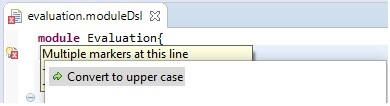
\includegraphics[scale=0.9]{\imageDir/validation-module-key-lower.jpg}
\caption{Modul \emph{key} muss \emph{upper case} sein}
\label{fig:validation-2}
\end{figure}

\begin{figure}[h]
\centering
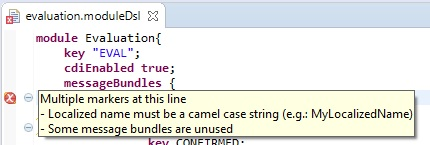
\includegraphics[scale=0.9]{\imageDir/validation-module-bundle.jpg}
\caption{MessageBundle name muss \emph{camel case} sein und sollte verwendet werden.}
\label{fig:validation-3}
\end{figure}
\ \newpage

\begin{figure}[h]
\centering
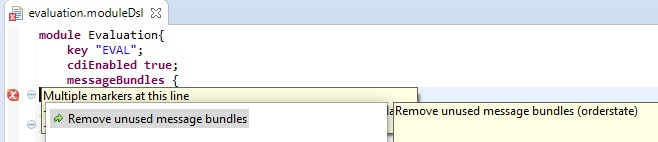
\includegraphics[scale=0.9]{\imageDir/validation-module-bundle-fix.jpg}
\caption{MessageBundle \emph{Quickfix} Optionen.}
\label{fig:validation-4}
\end{figure}

\begin{figure}[h]
\centering
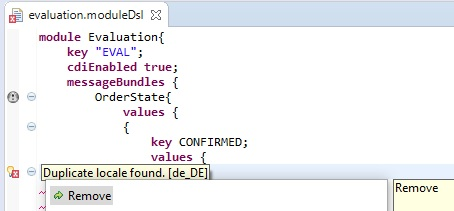
\includegraphics[scale=0.9]{\imageDir/validation-loc-entry-duplicate-locale.jpg}
\caption{Sprachspezifischer Eintrag mit doppeltet vergebener \emph{Locale}}
\label{fig:validation-5}
\end{figure}

\begin{figure}[h]
\centering
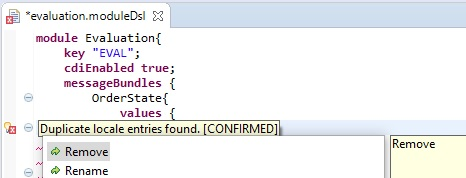
\includegraphics[scale=0.9]{\imageDir/validation-loc-entry-duplicate-key.jpg}
\caption{Sprachspezifischer Eintrag mit doppeltet vergebenen Schlüssel}
\label{fig:validation-6}
\end{figure}
\newpage

\begin{figure}[h]
	\centering
	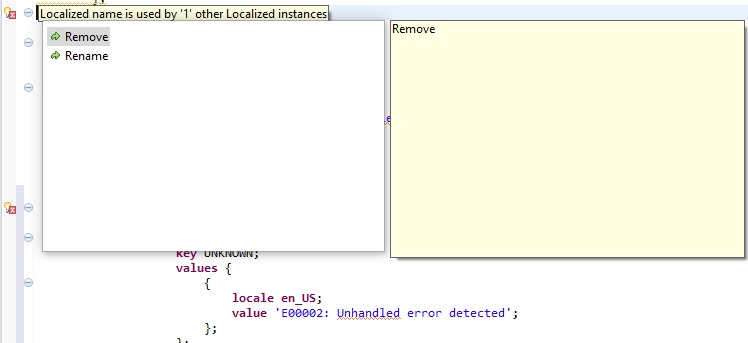
\includegraphics[scale=0.7]{\imageDir/validation-module-bundle-duplicate.jpg}
	\caption{Doppelter Name eines \emph{Localized}}
	\label{fig:validation-7}
\end{figure}

\begin{figure}[h]
	\centering
	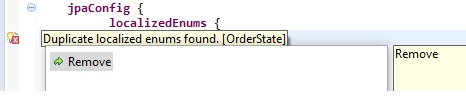
\includegraphics[scale=0.9]{\imageDir/validation-jpa-duplicate-bundle.jpg}
	\caption{\emph{JPA}-Konfiguration mit doppelten \emph{Localized}}
	\label{fig:validation-7}
\end{figure}

\begin{figure}[h]
	\centering
	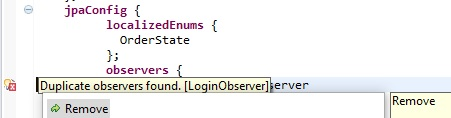
\includegraphics[scale=0.9]{\imageDir/validation-jpa-duplicate-observer.jpg}
	\caption{\emph{JPA}-Konfiguration mit doppelten \emph{Observer}}
	\label{fig:validation-8}
\end{figure}
\ \newpage


\begin{figure}[h]
	\centering
	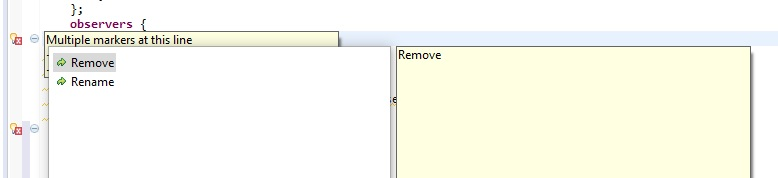
\includegraphics[scale=0.7]{\imageDir/validation-module-observer-duplicate.jpg}
	\caption{Doppelter Names eines \emph{Observers}}
	\label{fig:validation-9}
\end{figure}

\begin{figure}[h]
	\centering
	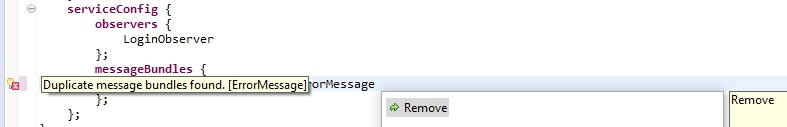
\includegraphics[scale=0.7]{\imageDir/validation-service-duplicate-bundle.jpg}
	\caption{\emph{Service}-Konfiguration mit doppelten \emph{Localized}}
	\label{fig:validation-10}
\end{figure}
	
\begin{figure}[h]
	\centering
	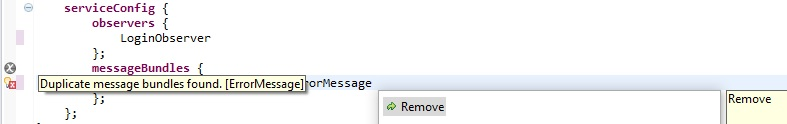
\includegraphics[scale=0.7]{\imageDir/validation-service-duplicate-observer.jpg}
	\caption{\emph{Service}-Konfiguration mit doppelten \emph{Observer}}
	\label{fig:validation-10}
\end{figure}
\ \newpage

\subsection{Generiert}
Für die Inhalte der generierten Ressourcen bitte die \emph{./dsl/evaluation.moduledsl} im Hauptprojekt dazu verwenden, um das Testmodul zu generieren.
\begin{figure}[h]
	\centering
	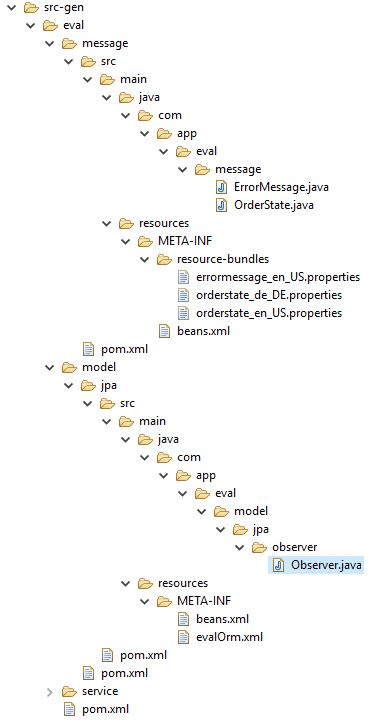
\includegraphics[scale=0.9]{\imageDir/generated_1.JPG}
	\caption{Erster Teil der generierten Ressourcen}
	\label{fig:generated-1}
\end{figure}
\ \newpage

\begin{figure}[h]
	\centering
	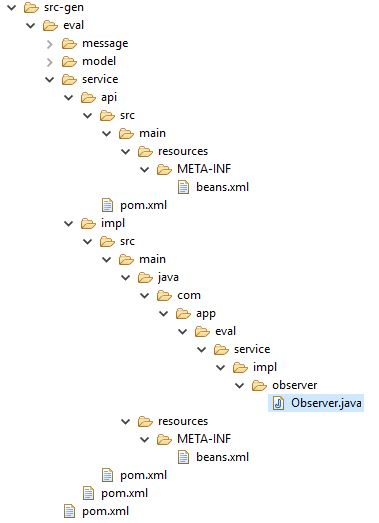
\includegraphics[scale=0.9]{\imageDir/generated_2.JPG}
	\caption{Zweiter Teil der generierten Ressourcen}
	\label{fig:generated-2}
\end{figure}
